\documentclass[border=10pt]{standalone}
\usepackage{tikz}
\usetikzlibrary{shapes, arrows.meta, positioning, fit, backgrounds}

\begin{document}
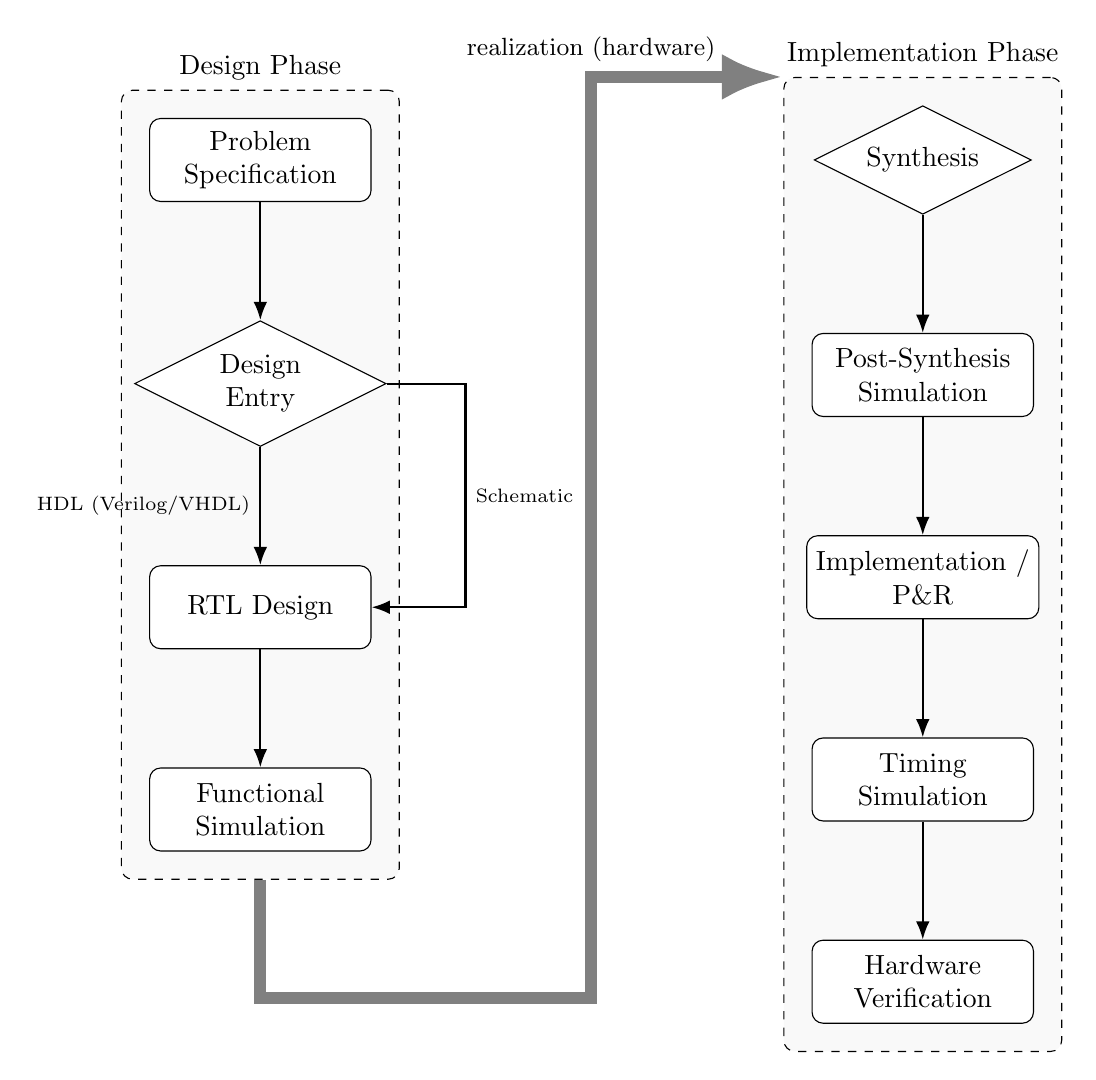
\begin{tikzpicture}[
    node distance=1.5cm and 2cm,
    block/.style={rectangle, draw, rounded corners, minimum height=3em, minimum width=8em, align=center, fill=white},
    decision/.style={diamond, draw, aspect=2, minimum height=3em, minimum width=6em, align=center, fill=white},
    arrow/.style={-Latex, thick},
    phase/.style={draw, dashed, rounded corners, inner sep=1em, fill=gray!5}
]

    % Design Phase Nodes
    \node[block] (problem) {Problem\\Specification};
    \node[decision, below=of problem] (design_entry) {Design\\Entry};
    \node[block, below=of design_entry] (rtl) {RTL Design};
    \node[block, below=of rtl] (func_sim) {Functional\\Simulation};

    % Design Phase Background
    \begin{scope}[on background layer]
        \node[phase, fit=(problem) (func_sim), label=above:Design Phase] (design_phase) {};
    \end{scope}

    % Edges within Design Phase
    \draw[arrow] (problem) -- (design_entry);
    \draw[arrow] (design_entry) -- node[left, font=\scriptsize] {HDL (Verilog/VHDL)} (rtl);
    \draw[arrow] (design_entry.east) -- ++(1,0) |- node[right, near start, font=\scriptsize] {Schematic} (rtl.east);
    \draw[arrow] (rtl) -- (func_sim);


    % Implementation Phase Nodes
    % Position Synthesis aligned with top of Implementation Phase, but shifted right
    \node[decision, right=7cm of problem, anchor=center] (synthesis) {Synthesis}; 
    % Align Synthesis somewhat centrally to the right of the design phase
    
    \node[block, below=of synthesis] (post_syn) {Post-Synthesis\\Simulation};
    \node[block, below=of post_syn] (impl) {Implementation /\\P\&R};
    \node[block, below=of impl] (timing) {Timing\\Simulation};
    \node[block, below=of timing] (hw_verif) {Hardware\\Verification};

    % Implementation Phase Background
    \begin{scope}[on background layer]
        \node[phase, fit=(synthesis) (hw_verif), label=above:Implementation Phase] (impl_phase) {};
    \end{scope}

    % Edges within Implementation Phase
    \draw[arrow] (synthesis) -- (post_syn);
    \draw[arrow] (post_syn) -- (impl);
    \draw[arrow] (impl) -- (timing);
    \draw[arrow] (timing) -- (hw_verif);

    % Transition between phases
    % "Design -- "realization (hardware)" ---> Implementation"
    % The arrow goes from Design Phase to Implementation Phase.
    % Let's connect Functional Simulation to Synthesis to represent the flow, 
    % or maintain the abstract "Phase to Phase" connection if preferred, 
    % but usually flow implies connecting the last step of one to the first of another.
    % The mermaid graph had: "Design -- "realization (hardware)" ---> Implementation"
    % connecting the subgraphs.
    % Let's draw a large arrow between the bounding boxes.
    
    \draw[arrow, line width=1.5mm, gray] (design_phase.south) |- ++(4.2,-1.5) |- node[above, font=\small, black] {realization (hardware)} (impl_phase.north west);

\end{tikzpicture}
\end{document}
